%
% user_manual.tex
%
% Copyright (C) 2019 by Gabriel Mariano Marcelino <gabriel.mm8@gmail.com>.
%
% Relatório final do Trabalho Final da Disciplina EEL510265.
%
% This work is licensed under the Creative Commons Attribution-ShareAlike 4.0
% International License. To view a copy of this license,
% visit http://creativecommons.org/licenses/by-sa/4.0/.
%

%
% \brief User manual appendix.
%
% \author Gabriel Mariano Marcelino <gabriel.mm8@gmail.com>
%
% \version 0.1.0
%
% \date 27/11/2019
%

\newpage

\section*{Manual do Usuário} \label{sec:user_manual}

Neste apêndice encontra um manual de usuário preliminar do sistema.

\subsection{Compilando o Código Fonte}

Para compilar o código fonte, há dois procedimentos diferentes (um para cada tipo de plataforma alvo). Para a versão a ser executada em um microcomputador, é necessário o compilador ``gcc''\footnote{Procedimento testado utilizando a versão 9.2.1.}. Com o compilador instalado, basta abrir um terminal na pasta onde encontra-se o código fonte e executar o comando ``\textit{make}'', como pode ser visto na \autoref{fig:cmd-make}.

\begin{figure}[!ht]
    \begin{center}
        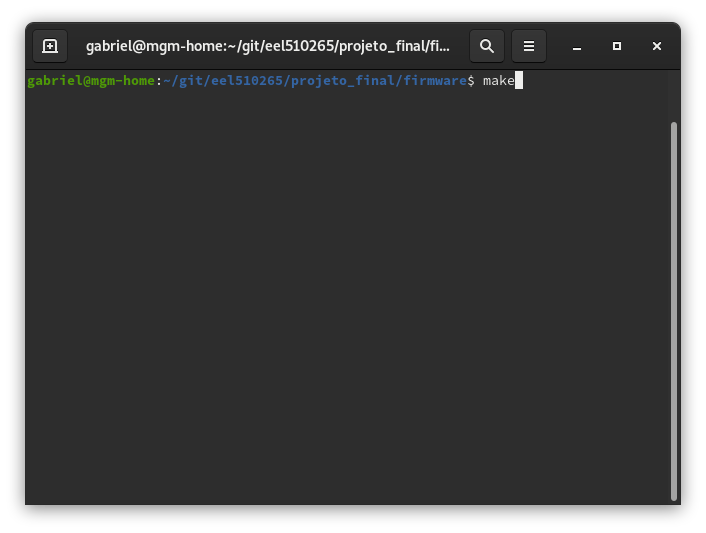
\includegraphics[width=0.75\textwidth]{figures/window_make.png}
        \caption{Terminal com o comando necessário para compilar o código fonte.}
        \label{fig:cmd-make}
    \end{center}
\end{figure}

\subsection{Executando o Código em um Microcomputador}

Após compilar o código fonte, para rodar o programa basta executar o comando:

\begin{itemize}
    \item ``\textit{./vending-machine}''
\end{itemize}

Este procedimento encontra-se ilustrado na \autoref{fig:cmd-exec}.

\begin{figure}[!ht]
    \begin{center}
        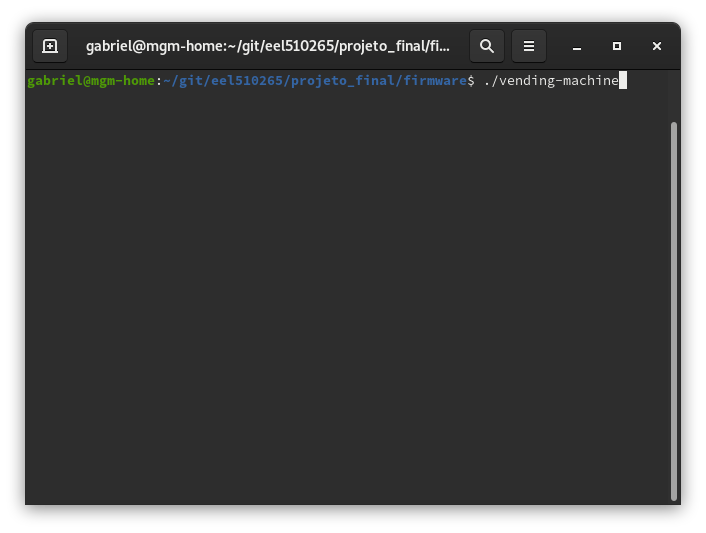
\includegraphics[width=0.75\textwidth]{figures/window-cmd-exec.png}
        \caption{Terminal com o comando necessário para executar o programa após a compilação.}
        \label{fig:cmd-exec}
    \end{center}
\end{figure}

\subsubsection{Tela inicial}

Logo após o comando de execução, o programa uma tela indicando o nome do mesmo e a versão do \textit{firmware}. Esta esta pode ser vista na \autoref{fig:splash-screen}.

\begin{figure}[!ht]
    \begin{center}
        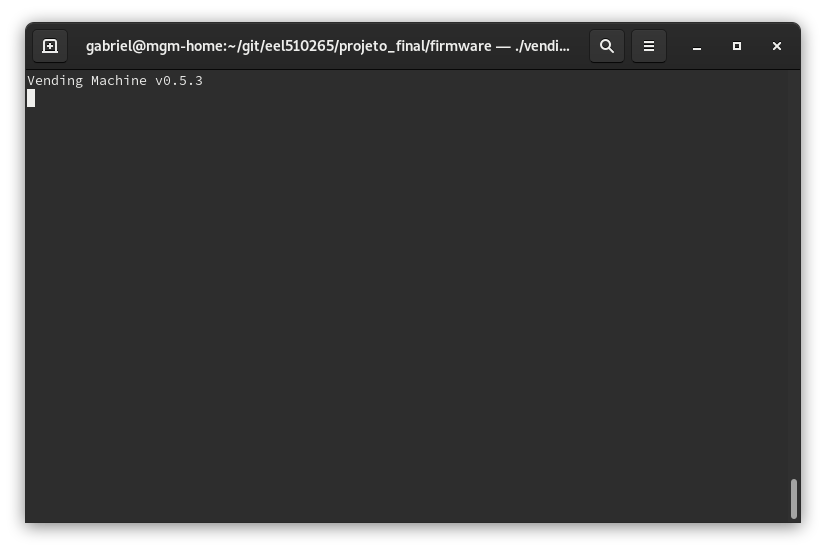
\includegraphics[width=0.75\textwidth]{figures/splash-screen.png}
        \caption{Tela de inicialização do programa.}
        \label{fig:splash-screen}
    \end{center}
\end{figure}

\subsubsection{Menu principal}

Após 2 segundos, a tela de inicialização é apagada e o menu principal é mostrado. Neste menu é possíve selecionar as duas opções de bebidas disponíveis. Para fazer essa seleção, basta digitar os números 1 ou 2 seguidos pela tecla \textit{enter}. Este menu pode ser visto na \autoref{fig:main-menu}.

\begin{figure}[!ht]
    \begin{center}
        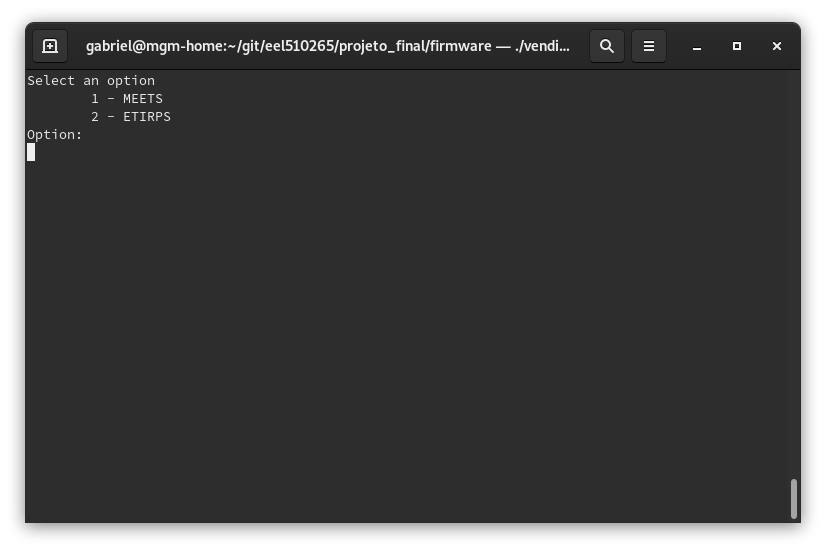
\includegraphics[width=0.75\textwidth]{figures/main-menu.png}
        \caption{Menu principal com as bebidas disponíveis.}
        \label{fig:main-menu}
    \end{center}
\end{figure}

\subsubsection{Inserção de Moedas}

Após escolher o tipo de bebida desejado, o nome e o preço da mesma aparecem na tela junto com instruções para inserir as moedas na máquina, como pode ser visto na \autoref{fig:drink-menu}.

\begin{figure}[!ht]
    \begin{center}
        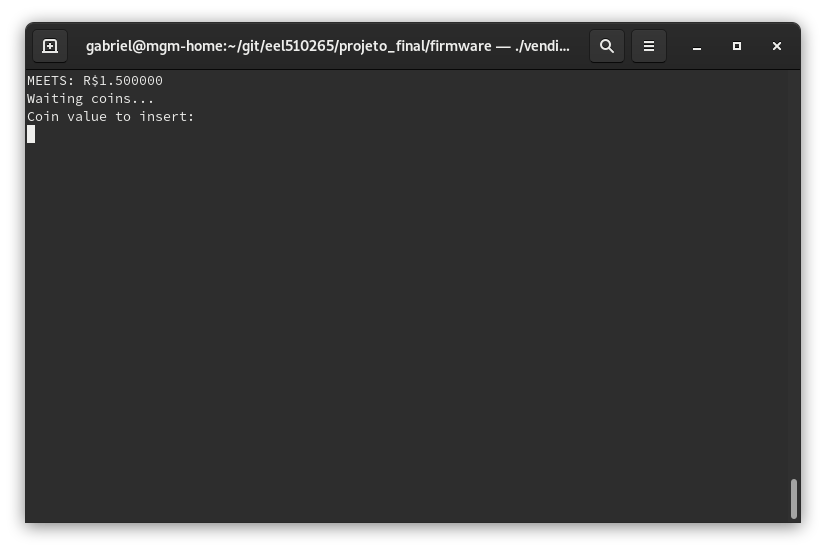
\includegraphics[width=0.75\textwidth]{figures/drink-menu.png}
        \caption{Terminal com o comando necessário para executar o programa após a compilação.}
        \label{fig:drink-menu}
    \end{center}
\end{figure}

Após o valor total da respectiva bebida ser inserido, a mesma é liberada pela máquina. Caso o usuário não insira nenhuma moeda por um período de 10 segundos, a operação a cancelada e as moedas já inseridas são devolvidas. Caso o usuário insira um valor superior ao da respectiva bebida, a mesma é liberada juntamente com o troco correspondente.

No caso de uma moeda inválida ser inserida, a mesma é devolvida logo após a inserção.

\subsubsection{Log de operações}

Para registrar as operações de venda, há um sistema de mensagens \textit{log} implementado. No caso da versão voltada para microcomputadores, as mensagens de \textit{log} são salvas em um arquivo CSV (\textit{Comma Separated Values}) a cada 5 segundos (caso haja uma operação de venda dentro deste período). As mensagens de log são compostas pela data e horário do evento e pelo nome da bebida correspondente ao evento.
